\documentclass{beamer}
%%%%%%%%%%%%%%%%%%%%%%%%%%%%%%%%%%%%%%%%%%%%%%%%%%%%%%%%%%%%%%%%%%%%%%%%%%%%
\usepackage{microtype}
%%% INCLUDE FILE FOR DEFINITIONS
%%% These may require various packages.

% Shortcuts in regular text
\newcommand{\degs}{\ensuremath{^\circ}}
\newcommand{\EE}[1]{\ensuremath{\times 10^{#1}}}
\newcommand{\ttimes}{\ensuremath{{}\times{}}}
\newcommand{\cclicense}{%
  \smash{\raisebox{-0.45ex}{%
  \setlength{\unitlength}{1em}%
  \begin{picture}(1,1)%
    \put(0.5,0.5){\circle{1}}
    \put(0.5,0.5){\hbox to 0pt{\hss\raisebox{-.45ex}{\tiny\textsf{CC}}\hss}}
  \end{picture}%
  }}%
  \hskip -1em%
  \href{http://creativecommons.org/licenses/by-nc-sa/3.0/}%
  {\ \hskip 1em \textsf{BY-NC-SA}}%
}

%\newcommand{\horizsep}{{\par\noindent\centering\rule[.25ex]{.75\columnwidth}{2pt}\par}}
\newcommand{\horizsep}{\vspace{\baselineskip}\noindent\hspace{\stretch{1}}$
\ast\qquad \ast\qquad \ast\qquad
$ \hspace{\stretch{1}} \vspace{\baselineskip}}
\newcommand{\pytrt}{\textsf{PyTRT}}

% Research
\newcommand{\lop}[1]{\mathcal{L}\!\left[#1\right]}
\newcommand{\lopinv}[2]{\mathcal{I}_{#1}\!\left[#2\right]}
\newcommand{\Dtens}{\mat{D}}
\newcommand{\Etens}{\mat{E}}
\newcommand{\Identitytens}{\mat{I}}
\newcommand{\APone}{AP$_1$}
\newcommand{\Pone}{P$_1$}
\newcommand{\SN}{S$_N$}%{S$_\text{N}$}%{$S_N$}%
\newcommand{\PN}{P$_N$}%{P$_\text{N}$}%{$P_N$}%
\newcommand{\CN}{Crank--Nicolson} %Yes, it's Nic not Nich
\newcommand{\Eddington}{\mathcal{E}} %whatever symbol I decided for Eddington
\newcommand{\RadEn}{E} %whatever symbol I decide for radiation energy
\newcommand{\Sigmatr}{\Sigma_{\mathit{tr}}}

% Program names
\newcommand{\cpp}{\textsf{C\raisebox{0.2ex}{++}}}

% General math shortcuts
\newcommand{\ud}{\mathop{}\!\mathrm{d}}
\newcommand{\pder}[2]{\frac{\partial #1}{\partial #2}}
\newcommand{\oder}[2]{\frac{\mathrm{d} #1}{\mathrm{d} #2}}
\newcommand{\tpder}[2]{{\partial #1}/{\partial #2}} %inlined
\newcommand{\toder}[2]{{\mathrm{d} #1}/{\mathrm{d} #2}} %inlined
\newcommand{\lra}{ \quad \Longrightarrow \quad }
\newcommand{\eexp}{\mathop{}\!\mathrm{e}} % upright ``e'' for exponent
\newcommand{\expp}[1]{\exp\!\left( {#1} \right)} % exp with parentheses
\newcommand{\qeq}{\stackrel{\mathrm{?}}{=}}

% Probability
\newcommand{\expectation}[1]{\mathop{}\!\mathrm{E}\!\left[ #1 \right]}
\DeclareMathOperator{\Var}{Var} % variance

% Asymptotic analysis
\DeclareMathOperator{\Ei}{Ei} % Exponential function
\newcommand{\lapl}[1]{\mathcal{L}[{#1}]} %laplace

%change the Re and Im operators from fancy curly letters
\DeclareMathOperator{\MathOpRe}{Re}
\renewcommand{\Re}{\MathOpRe}
\DeclareMathOperator{\MathOpIm}{Im}
\renewcommand{\Im}{\MathOpIm}

%imaginary ``i'' , upright 'i' or \imath
\newcommand{\iimag}{\mathrm{i}}

% Finite differences
\newcommand{\hot}{\text{h.o.t.}}
\newcommand{\inv}{^{-1}}

% Numerical Linear Algebra
\newcommand{\conj}{^{\ast}} % complex conjugate (transpose)
\newcommand{\norm}[1]{\left\| #1 \right\|} % double pipe
\newcommand{\abs}[1]{\left| #1 \right|} % single pipe
\newcommand{\eps}{\varepsilon}
\DeclareMathOperator{\fl}{fl}

\DeclareMathOperator{\acosh}{arccosh} 

% Define a command to write a nice-looking element, e.g. 4,2 He
\newcommand{\elem}[3]{\ensuremath{{}^{{#1}}_{{#2}}\mathrm{{#3}}}}

% Vector definitions
\newcommand{\mat}[1]{\mathbf{#1}} %matrix is bold upright
\renewcommand{\vec}[1]{\bm{#1}} %vector is bold italic
\newcommand{\op}[1]{\mathsf{#1}} % ``operator'' is sans serif

\newcommand{\vd}{\bm{\cdot}} % slightly bold vector dot
\newcommand{\del}{\vec{\nabla}} % gradient (Del) is bold
\newcommand{\grad}{\vec{\nabla}} % gradient

%\newcommand{\abr}[1]{\langle {#1} \rangle}
\newcommand{\abr}[1]{\left\langle {#1} \right\rangle} % angle brackets for avg.

%% topbox is useful in extended definitions of math terms inside an align
\newcommand{\topbox}[2][0.6]{\parbox[t]{#1\columnwidth}{\raggedright{}#2}}

% commands to make text in math mode appear as zero-width (better-looking
% integrals/sums, e.g.)
% from mathmode.pdf page 74, or Alexander R. Perlis ``A complement to \smash,
% \llap, and \rlap''

\def\mathllap{\mathpalette\mathllapinternal}
	\def\mathllapinternal#1#2{%
	\llap{$\mathsurround=0pt#1{#2}$}%
}
\def\clap#1{\hbox to 0pt{\hss#1\hss}}%
\def\mathclap{\mathpalette\mathclapinternal}%
\def\mathclapinternal#1#2{%
	\clap{$\mathsurround=0pt#1{#2}$}%
}
\def\mathrlap{\mathpalette\mathrlapinternal}%
\def\mathrlapinternal#1#2{%
	\rlap{$\mathsurround=0pt#1{#2}$}%
}

\setSRJthesisfigurepaths

%%%%%%%%%%%%%%%%%%%%%%%%%%%%%%%%%%%%%%%%%%%%%%%%%%%%%%%%%%%%%%%%%%%%%%%%%%%%

%30 minute presentation
%15 minutes scheduled for questions
%1 hour allotted total

\usetheme{AnnArbor}
\usecolortheme{seahorse}
\usecolortheme{orchid}
\usefonttheme[onlymath]{serif}
\setbeamercolor*{frametitle}{use=structure,bg=structure.fg!20!white}
\setbeamercolor*{frametitle right}{use=structure,bg=structure.fg!20!white}
%\setbeamertemplate{navigation symbols}{\insertframenavigationsymbol}
\setbeamertemplate{caption}[numbered]

\title[PyTRT]%
{PyTRT: a Python/C++ framework for transport methods development}

\author[SRJ]{Seth~Johnson}

\institute[UMich]{
University of Michigan, Ann Arbor
}
\date[5/6/2011]{May 6, 2011}

\AtBeginSection[]
{
\begin{frame}
  \frametitle{Outline}
  \tableofcontents[currentsection]
\end{frame}
}

\hypersetup{colorlinks=true,linkcolor=black}

%use symbols for footnote
\renewcommand{\thefootnote}{\fnsymbol{footnote}}

\begin{document}
%%%%%%%%%%%%%%%%%%%%%%%%%%%%%%%%%%%%%%%%%%%%%%%%%%%%%%%%%%%%%%%%%%%%%%%%%%%%

\begin{frame}
\titlepage
\vspace{-.25in}
\begin{center}
  
\includegraphics[width=0.5\textwidth]{logo}
  \hspace{.5in}
  
\includegraphics[width=0.2\textwidth]{umlogo}
\end{center}
\smash{
\includegraphics[width=0.2\textwidth]{neup-small}}
\end{frame}

%%%%%%%%%%%%%%%%%%%%%%%%%%%%%%%%%%%%%%%%%%%%%%%%%%%%%%%%%%%%%%%%%%%%%%%%%%%%
\section{Introduction}
%%%%%%%%%%%%%%%%%%%%%%%%%%%%%%%%%%%%%%%%
\begin{frame}{Design goals}
\begin{block}{Primary mission}
   To graduate in a timely manner.
\end{block}


\begin{itemize}
  \item rapid, error-free implementation of new methods,
  \item easy definition of multiple-method test problems,
  \item high-performance solver kernels to run the problems quickly,
  \item powerful data analysis tools driven by user needs (me), and
  \item automated generation of high-quality figures.
\end{itemize}
  
\end{frame}

%%%%%%%%%%%%%%%%%%%%%%%%%%%%%%%%%%%%%%%%
\begin{frame}{Capabilities}
Cartesian product of methods:
\begin{itemize}
  \item Steady-state, linear time-dependent, and nonlinear (semi-implicit)
    TRT
  \item 1-D, Flatland, 2-D
  \item Monte Carlo, \SN\ transport, diffusion, \Pone, anisotropic diffusion
\end{itemize}

Analysis:
\begin{itemize}
  \item Lineout
  \item Angleout
  \item Matrixout
  \item Silo for VisIT
\end{itemize}
  
\end{frame}

%%%%%%%%%%%%%%%%%%%%%%%%%%%%%%%%%%%%%%%%
\begin{frame}{Techniques}
Reliability:
\begin{itemize}
  \item CMake build process
  \item Git for version control
  \item Unit tests (regression)
  \item Design By Contract
  \item Modular design
  \item Trilinos for linear algebra\footnote{Two-edged sword in terms of
    reliability}
\end{itemize}

Code reuse:
\begin{itemize}
  \item Template on geometry, etc.
  \item Python wrapper handles linearization
  \item Python handles all the stuff that only needs to happen once
\end{itemize}
  
\end{frame}

%%%%%%%%%%%%%%%%%%%%%%%%%%%%%%%%%%%%%%%%
\begin{frame}{Modular design}

{\centering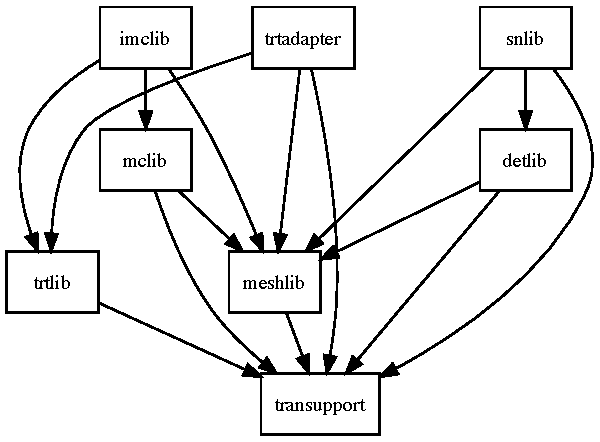
\includegraphics[height=2.75in]{hierarchy}\par}

\end{frame}

%%%%%%%%%%%%%%%%%%%%%%%%%%%%%%%%%%%%%%%%%%%%%%%%%%%%%%%%%%%%%%%%%%%%%%%%%%%%
\section{Object-oriented boundary conditions}
%%%%%%%%%%%%%%%%%%%%%%%%%%%%%%%%%%%%%%%%
\begin{frame}[fragile]{Object oriented boundary conditions}
  \begin{itemize}
\item Abstract \verb|BoundaryCondition| class:
  \begin{itemize}
    \item At least one \verb|apply| method
    \item Other methods like \verb|getIncidentSourceRate|
  \end{itemize}

\item Generic \verb|BcManager| class:
  \begin{itemize}
    \item The problem definition contains a \verb|BcManager| object
    \item Vector that maps \verb|BoundaryFace| to \verb|BoundaryCondition*|
    \item Functors to help with modifying multiple boundary conditions
  \end{itemize}
\end{itemize}
\end{frame}

%%%%%%%%%%%%%%%%%%%%%%%%%%%%%%%%%%%%%%%%
\begin{frame}[fragile]{Diffusion/constructed matrix}
  \begin{verbatim}
void MyBc::apply(const BoundaryFaceT& bface,
                 ProxyVector& vec) const
{
    const CellT& cell = *insideBoundaryCell(&bface);
    source.getFlux()[ cell ] += /* some value */;
}

void apply(const BoundaryFaceT& bface,
           Operator& matrix) const
{
    const CellT& cell = *insideBoundaryCell(&bface);
    matrix.startRow( matrix.getFlux()[cell] );
    matrix.pushRowElement( matrix.getFlux()[cell], /*val*/);
    matrix.finishRow();
}
  \end{verbatim}
\end{frame}

\begin{frame}[fragile]{Diffusion/constructed matrix}
Called after initializing source vector:
\begin{verbatim}
	bcs.apply( <Traits::BcManagerT, ProxyVector>(sourceVec) );
\end{verbatim}
  
Called after the internal part of the diffusion matrix has been built:
\begin{verbatim}
  startMatrix( ACCUMULATE );
  bcs.apply(BcOperatorApplier<Traits>(*this));
  finishMatrix();
\end{verbatim}
\end{frame}

%%%%%%%%%%%%%%%%%%%%%%%%%%%%%%%%%%%%%%%%
\begin{frame}[fragile]{\SN\ boundary conditions}
  \begin{verbatim}
void ReflectingBoundaryCondition::apply(
        const BoundaryFaceT& bface,
        Vector& source ) const
{
    bool onNegBoundary = bface.getFace()->onNegBoundary();
    unsigned int axis = bface.getFace()->getAxis();
    FluxDiscreteT& sourceFlux = source.getBoundaryFlux()[ bface ];
    for (QuadratureSetT::const_iterator angle = qs_.begin();
            angle != qs_.end(); ++angle)
    {
        if (isPositive(angle->getOmega()[axis]) == onNegBoundary ) {
            sourceFlux[ *angle ]
                = sourceFlux[ qs_.getReflectedAngle(*angle, axis) ];
        }
    }
}
  \end{verbatim}
\end{frame}

%%%%%%%%%%%%%%%%%%%%%%%%%%%%%%%%%%%%%%%%
\begin{frame}[fragile]{MC boundary conditions}
  \begin{verbatim}
template<class ProblemTraits_T>
void VacuumBoundaryCondition<ProblemTraits_T>::apply(
        const BoundaryFaceT& bface,
        ParticleT& particle,
        Tally& tally) const
{
    tally.particleExited( bface, particle );
    particle.markDestroyed();
}
  \end{verbatim}
\end{frame}

%%%%%%%%%%%%%%%%%%%%%%%%%%%%%%%%%%%%%%%%%%%%%%%%%%%%%%%%%%%%%%%%%%%%%%%%%%%%
\section{Python}
\begin{frame}[fragile]{Python structure}
  \begin{itemize}
    \item \verb|Manager| class emits \cpp\ problem depending on module passed
      to it (duck typing)
    \item \verb|Solver| handles time stepping, callbacks, user feedback, etc.
    \item Callbacks include Silo output, liveplot, lineout, angleout, MC
      particle tally info, $\Delta t$ vs. $t$, etc.
    \item Lineout etc. use PyTables to store HDF5 data and metadata
  \end{itemize}

  High-level ``glue'' written in Python:
  \begin{itemize}
    \item Flux-limited diffusion
    \item Linearization scheme
    \item Multigrid management
    \item Time-dependent ``events''
  \end{itemize}
\end{frame}

\begin{frame}{Angleout}

{\centering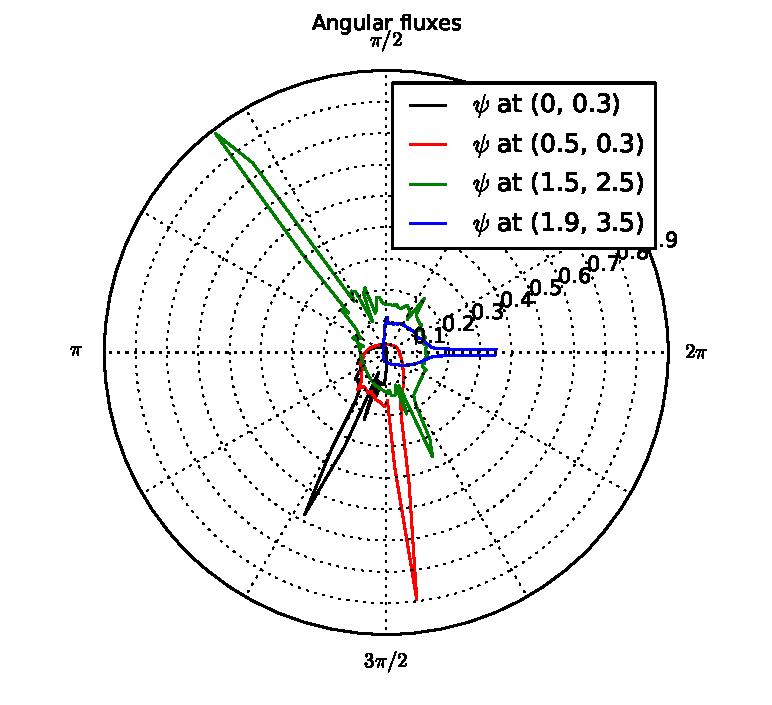
\includegraphics[height=2.75in]{angleout}\par}
\end{frame}

%%%%%%%%%%%%%%%%%%%%%%%%%%%%%%%%%%%%%%%%%%%%%%%%%%%%%%%%%%%%%%%%%%%%%%%%%%%%
\section{Conclusions}
%%%%%%%%%%%%%%%%%%%%%%%%%%%%%%%%%%%%%%%%
\begin{frame}{Availability}

\begin{center}
Sponsored by the public, available to the public. (Simplified BSD license.)
\vspace{.5in}
  \Huge pytrt.org
\end{center}

\end{frame}

%%%%%%%%%%%%%%%%%%%%%%%%%%%%%%%%%%%%%%%%
\begin{frame}{Questions?}

{\centering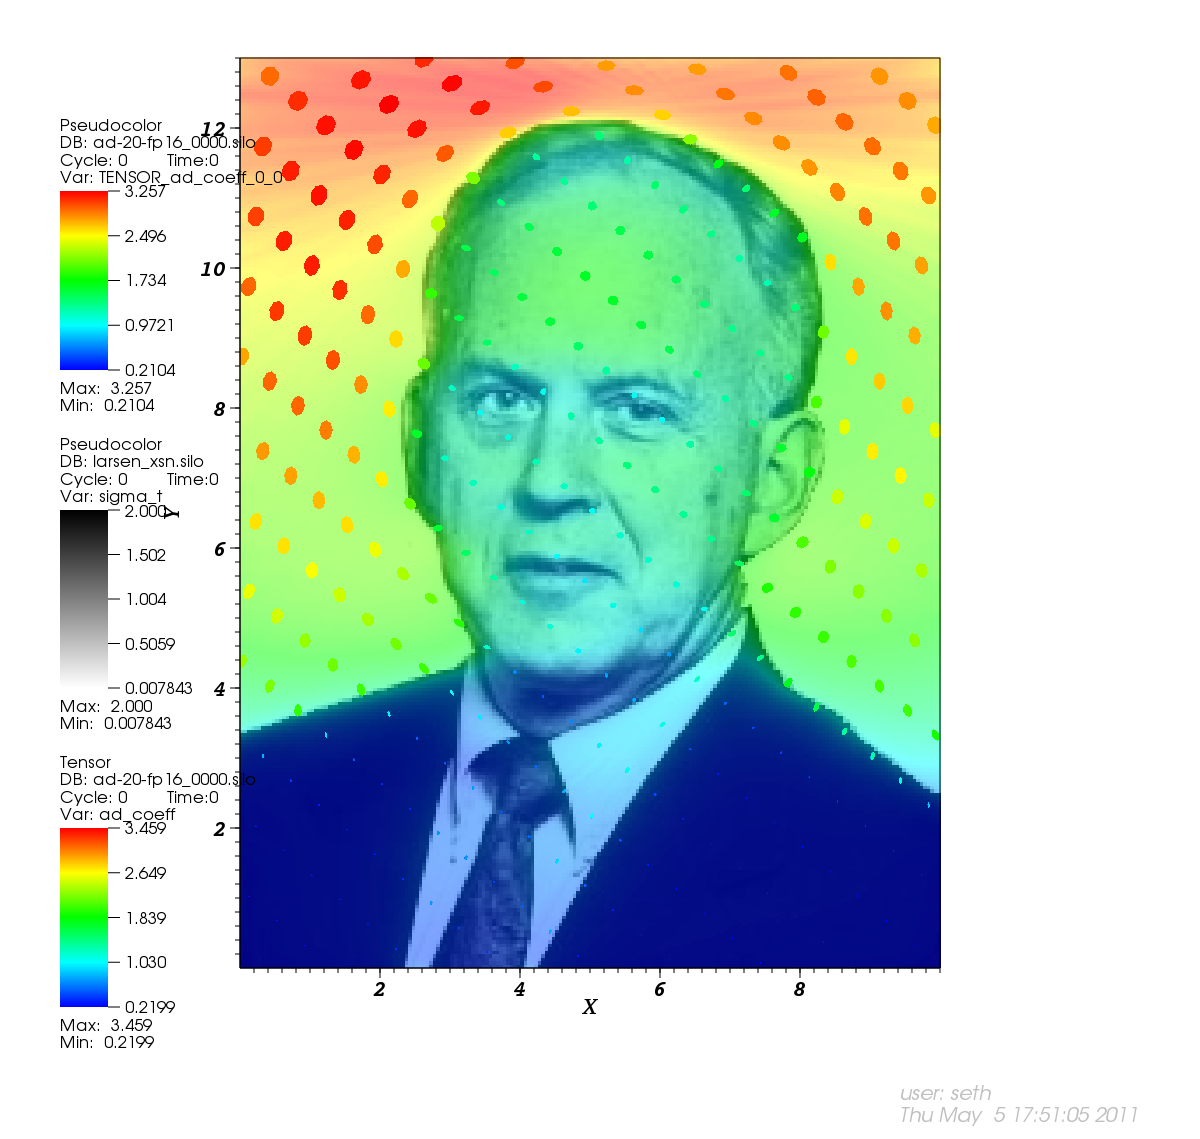
\includegraphics[height=2.75in]{larsen}\par}
\vspace{-\baselineskip}
{\setlength{\baselineskip}{-\baselineskip} \tiny 
This material is based upon work supported under a National Science Foundation
Graduate Research Fellowship and a Department of Energy Nuclear Energy
University Programs Graduate Fellowship. Any opinions, findings, conclusions or
recommendations expressed in this publication are those of the author and do
not necessarily reflect the views of the National Science Foundation or the
Department of Energy Office of Nuclear Energy.\par}
\end{frame}

%%%%%%%%%%%%%%%%%%%%%%%%%%%%%%%%%%%%%%%%%%%%%%%%%%%%%%%%%%%%%%%%%%%%%%%%%%%

%	This material is based upon work supported under a National Science
%	Foundation Graduate Research Fellowship. Any opinions, findings, conclusions
%	or recommendations expressed in this publication are those of the author(s)
%	and do not necessarily reflect the views of the National Science
%	Foundation.  
\end{document}
